\section{Numerical Results}
%%%%%%%%%%%%%%%%%%%%%%%%%%%%%%%%
%%%%%%%%%%%%%%%%%%%%%%%%%%%%%%%%
% Elongational flow
%%%%%%%%%%%%%%%%%%%%%%%%%%%%%%%%
%%%%%%%%%%%%%%%%%%%%%%%%%%%%%%%%

\begin{frame}{Numerical Results}
	\centering
	Elongational flow
\end{frame}


\begin{frame}{Elongational flow}
	\scriptsize
	Consider
	\begin{align*}
		\nabla_{\vec{x}} \vec{u}_{\mathrm{ext}}=\left(\begin{array}{ccc}
			2 & 0 & 0 \\
			0 & -1 & 0 \\
			0 & 0 & -1
		\end{array}\right) %, \text{for $\ell = 1, -1$}.
	\end{align*}
	
	Exact steady-state solution
	\begin{align}
		f_{\text {exact}}(\phi, \theta)=C_1 \exp \left(-\frac{3}{2 D_{\mathrm{r}}}\left(1-\cos ^2(\phi) \sin ^2(\theta)\right)\right),
	\end{align}
	with the constants $C_1 = 2.30121384511755303190$ for $D_r=0.1$.
	
	\begin{figure}
		%	\small
		%Solution on $S^2$
		\begin{minipage}{0.4\textwidth}
			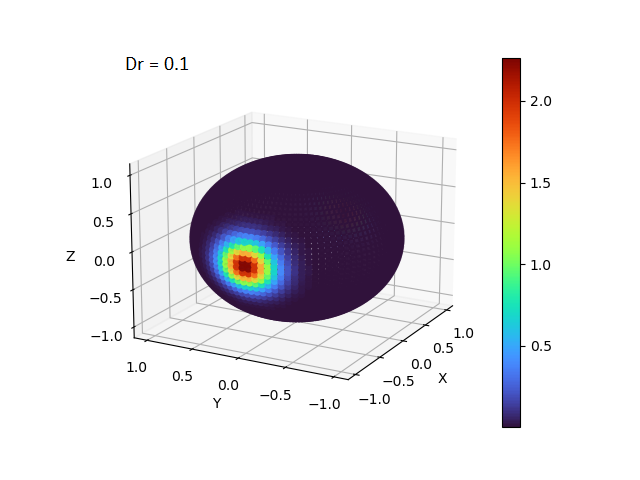
\includegraphics[scale=0.35]{Bilder/exakteLsg_example3.1}
		\end{minipage}
		\hfill 
		\begin{minipage}{0.4\textwidth}
			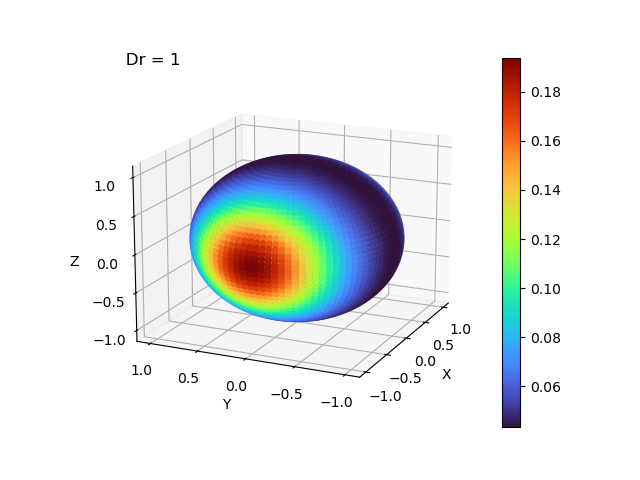
\includegraphics[scale=0.35]{Bilder/exakteLsg_example31_l=1_dr1}
		\end{minipage}
		\caption{Exact steady state solution with different $D_r$}
	\end{figure}
	
\end{frame}



\begin{frame}{Elongational flow}
	\begin{figure}
		\begin{minipage}{0.48\textwidth}
			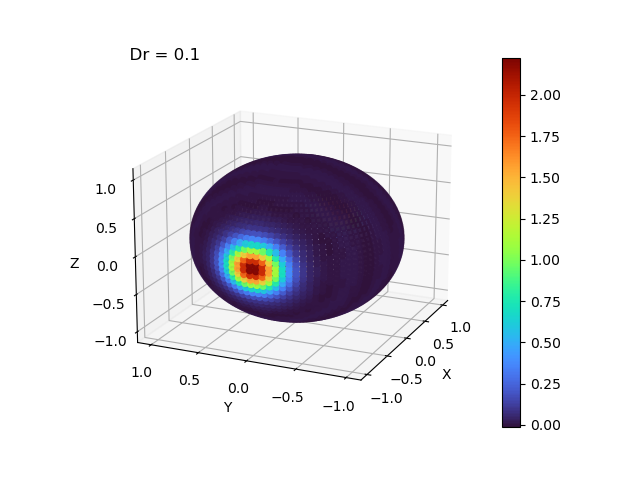
\includegraphics[scale=0.4]{Bilder/example3.1_14nd_linspace(0,10,500)_dr=0.1}
		\end{minipage}
		\hfill 
		\begin{minipage}{0.48\textwidth}
			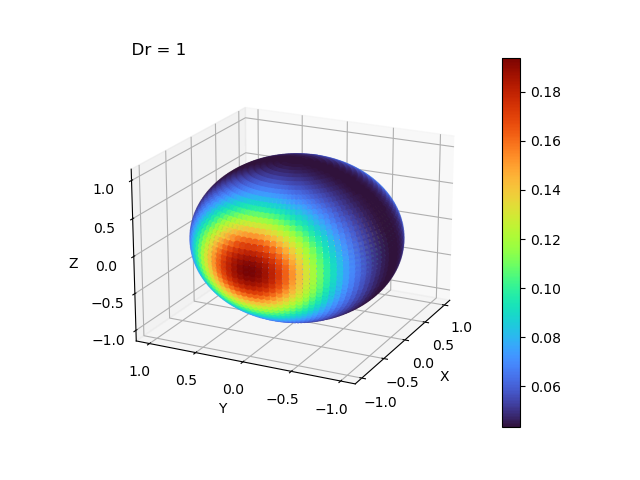
\includegraphics[scale=0.4]{Bilder/example3.1_14nd_linspace(0,10,1000)_dr=1}
		\end{minipage}
		\caption{Numerical solution on $S^2$ with basis functions of $14th.$ order}
	\end{figure}
\end{frame}

\begin{frame}{Convergence Study}
	For the convergence study, the maximum norm error is used
	\begin{align*}
		E_{max} = max|U_{exact} - U_{approx}|.
	\end{align*}
	
	\begin{figure}
		\begin{minipage}{0.45\textwidth}
			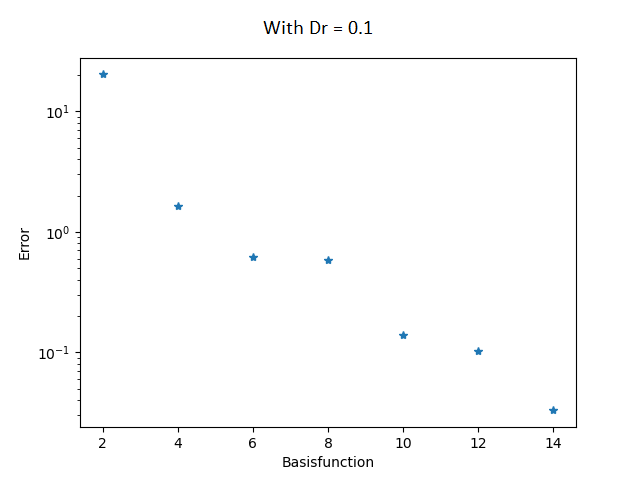
\includegraphics[scale=0.42]{Bilder/Konvergenzstudie_maxnorm_dr=0.1_l=1}
		\end{minipage}
		\hfill 
		\begin{minipage}{0.45\textwidth}
			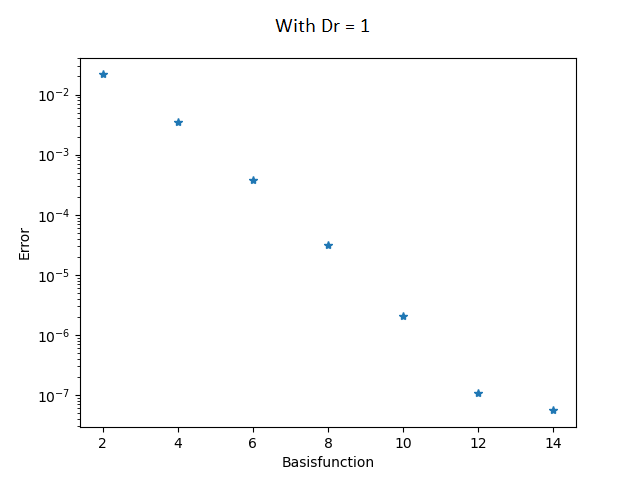
\includegraphics[scale=0.42]{Bilder/Konvergenzstudie_maxnorm_dr=1_l=1}
		\end{minipage}
		\caption{Error with respect to basisfunction with different $D_r$}
	\end{figure}
\end{frame}

%%%%%%%%%%%%%%%%%%%%%%%%%
% Stability analysis
%%%%%%%%%%%%%%%%%%%%%%%%%

\begin{frame}{Stability analysis}
	\begin{figure}
		\centering
		\subfloat[Coefficients as function]{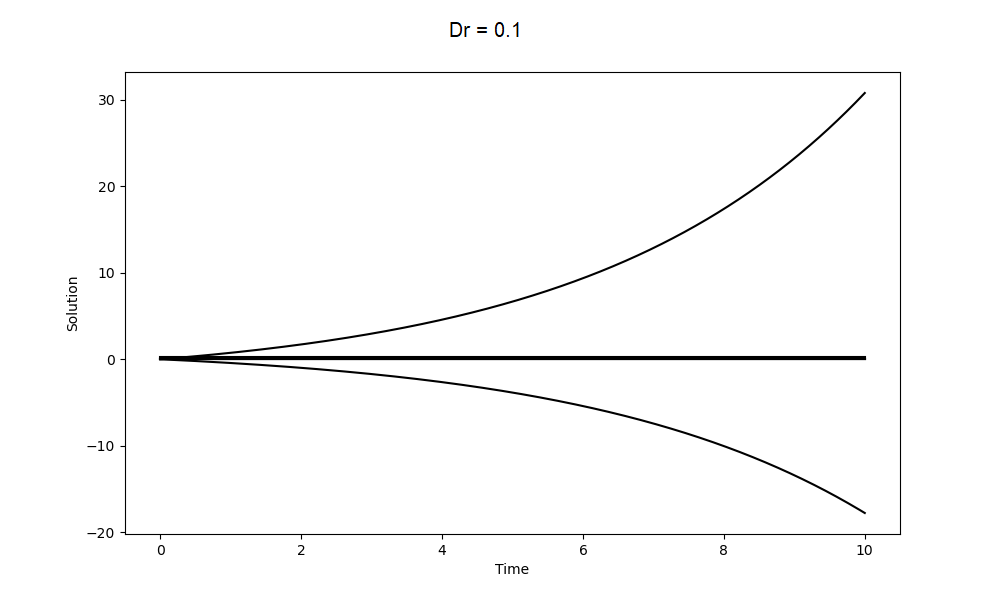
\includegraphics[width=5.5cm,height=4cm]{Bilder/elongational_l=1_lsg_ueber_Zeit_2nd}}
		\qquad
		\subfloat[Eigenvalue]{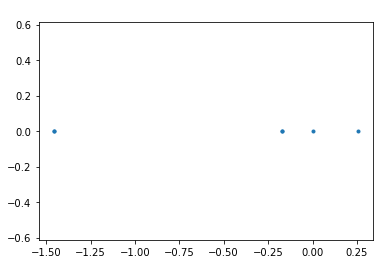
\includegraphics[width=5.5cm,height=3.8cm]{Bilder/Stability_analysis_2nd_dr0.1}}
		\caption{With $2nd$ order and $D_r$ = 0.1}
	\end{figure}
\end{frame}

\begin{frame}{Stability analysis: Eigenvalue with small $D_r$}
	\begin{figure}
		\begin{subfigure}{0.48\textwidth}
			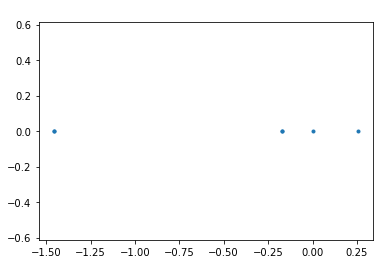
\includegraphics[width=\linewidth]{Bilder/Stability_analysis_2nd_dr0.1}
		\end{subfigure}
		\hfill
		\begin{subfigure}{0.48\textwidth}
			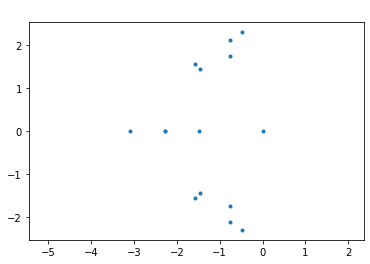
\includegraphics[width=\linewidth]{Bilder/Stability_analysis_4th_dr0.1}
		\end{subfigure}
		\caption{Eigenvalue of matrix $A$ with $D_r = 0.1$}
	\end{figure}

	\begin{block}{Finding}
		Eigenvalue for matrix of $2nd$ order ODE systems $>0$ $\Rightarrow$ method unstable
	\end{block}
\end{frame}

\begin{frame}{Stability analysis: Eigenvalue with small $D_r$}
	\begin{figure}
		\begin{subfigure}{0.48\textwidth}
			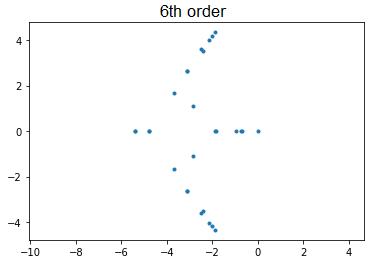
\includegraphics[width=\linewidth]{Bilder/Stability_analysis_6th_dr0.1}
		\end{subfigure}
		\hfill
		\begin{subfigure}{0.48\textwidth}
			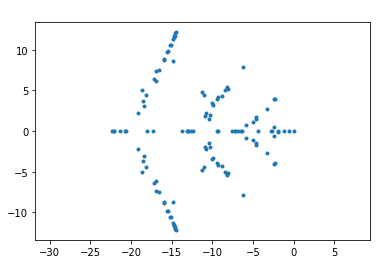
\includegraphics[width=\linewidth]{Bilder/Stability_analysis_14th_dr0.1}
		\end{subfigure}
		\caption{Eigenvalue of matrix $A$ with $D_r = 0.1$}
	\end{figure}
\end{frame}

\begin{frame}{Stability analysis: Eigenvalue with large $D_r$}
	\begin{figure}
		\begin{subfigure}{0.48\textwidth}
			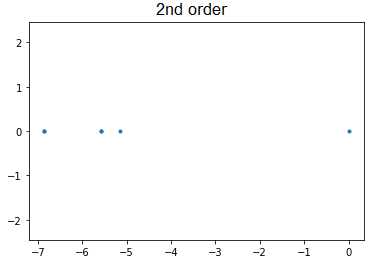
\includegraphics[width=\linewidth]{Bilder/Stability_analysis_2nd_dr1}
		\end{subfigure}
		\hfill
		\begin{subfigure}{0.48\textwidth}
			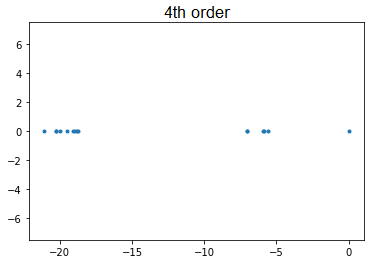
\includegraphics[width=\linewidth]{Bilder/Stability_analysis_4th_dr1}
		\end{subfigure}
		\caption{Eigenvalue of matrix $A$ with $D_r = 1$}
	\end{figure}
\end{frame}

\begin{frame}{Absolute stability: for large $D_r$}
	\begin{figure}
		\begin{subfigure}{0.48\textwidth}
			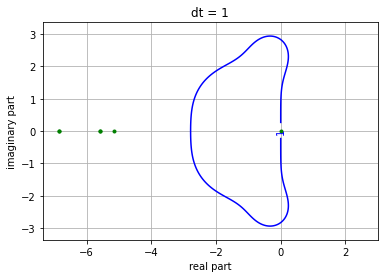
\includegraphics[width=\linewidth]{Bilder/RK4_region_2nd_dr=1_dt=1}
		\end{subfigure}
		\hfill
		\begin{subfigure}{0.48\textwidth}
			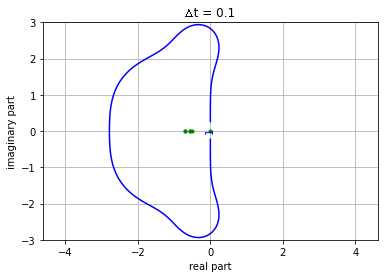
\includegraphics[width=\linewidth]{Bilder/RK4_region_2nd_dr=1_dt=0.1}
		\end{subfigure}
		\caption{Stability region $RK4$ with eigenvalue of $2nd$ order ODE systems with $Dr=1$ and different time steps}
	\end{figure}
\end{frame}

\begin{frame}{Absolute stability: for large $D_r$}
	\begin{figure}
		\begin{subfigure}{0.48\textwidth}
			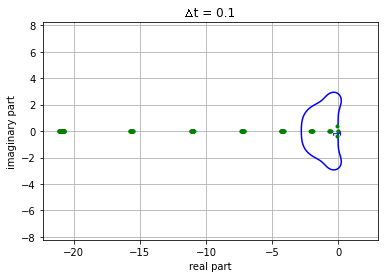
\includegraphics[width=\linewidth]{Bilder/RK4_region_14th_dr=1_dt=0.1}
		\end{subfigure}
		\hfill
		\begin{subfigure}{0.48\textwidth}
			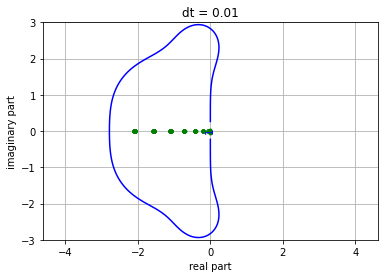
\includegraphics[width=\linewidth]{Bilder/RK4_region_14th_dr=1_dt=0.01}
		\end{subfigure}
		\caption{Stability region $RK4$ with eigenvalue of $14th$ order ODE systems with $Dr=1$ and different time steps}
	\end{figure}

	\begin{block}{Finding}
	For absolute stability for large $D_r$  $\rightarrow$ smaller time steps is needed
	\end{block}
\end{frame}


\begin{frame}{Coefficients as function}
	\begin{figure}
		\begin{subfigure}{0.48\textwidth}
			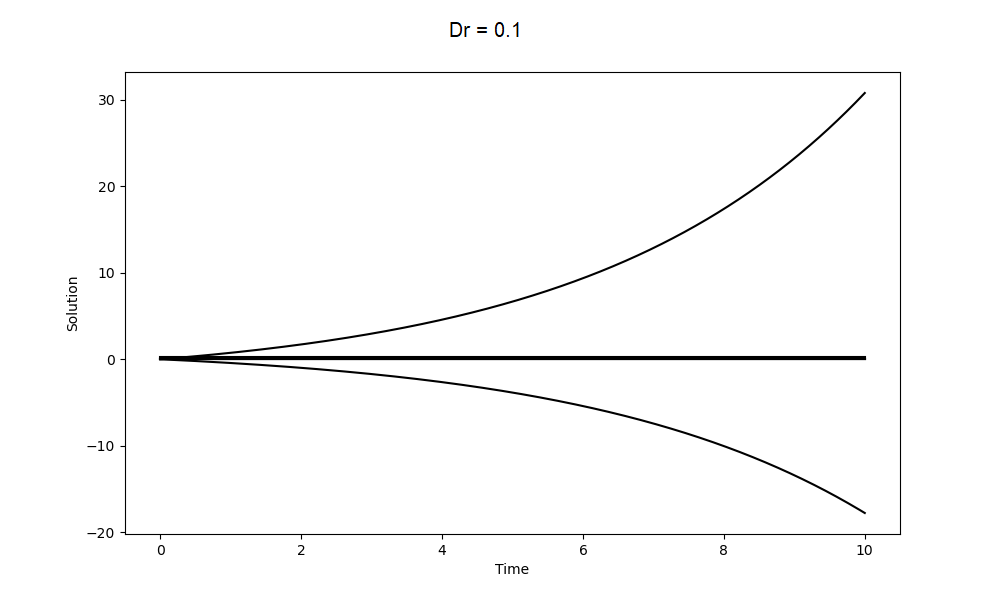
\includegraphics[width=\linewidth]{Bilder/elongational_l=1_lsg_ueber_Zeit_2nd}
		\end{subfigure}
		\hfill
		\begin{subfigure}{0.48\textwidth}
			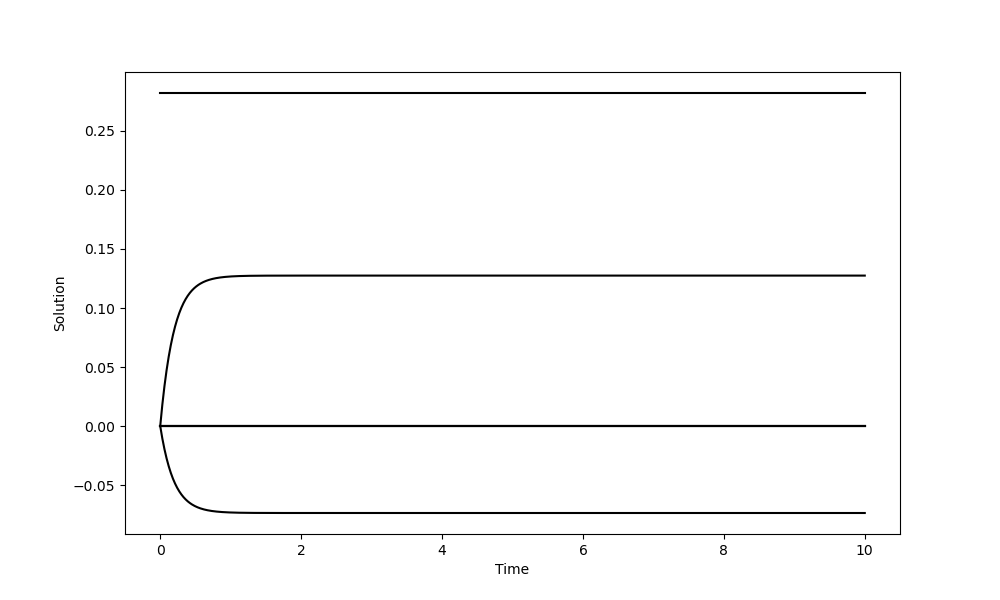
\includegraphics[width=\linewidth]{Bilder/elongational_l=1_lsg_ueber_Zeit_2nd_dr=1}
		\end{subfigure}
		\caption{Coefficients as function of $2nd$ order}
	\end{figure}
\end{frame}


\begin{frame}{Coefficients as function}
	\begin{figure}
		\begin{subfigure}{0.48\textwidth}
			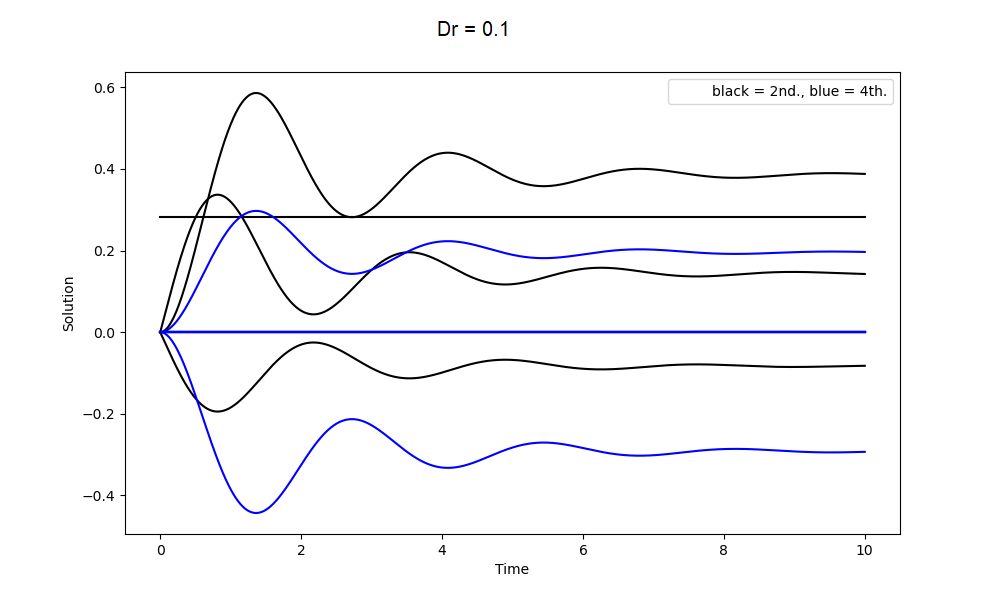
\includegraphics[width=\linewidth]{Bilder/elongational_l=1_lsg_ueber_Zeit_4th}
		\end{subfigure}
		\hfill
		\begin{subfigure}{0.48\textwidth}
			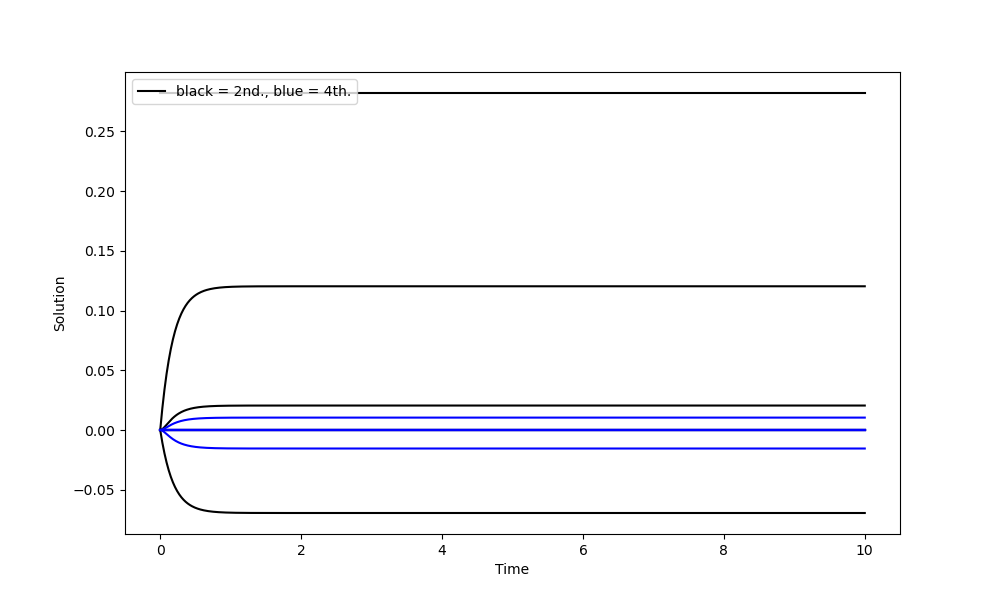
\includegraphics[width=\linewidth]{Bilder/elongational_l=1_lsg_ueber_Zeit_4th_dr=1}
		\end{subfigure}
		\caption{Coefficients as function of $4th$ order}
	\end{figure}
\end{frame}


\begin{frame}{Coefficients as function}
	\begin{figure}
		\begin{subfigure}{0.48\textwidth}
			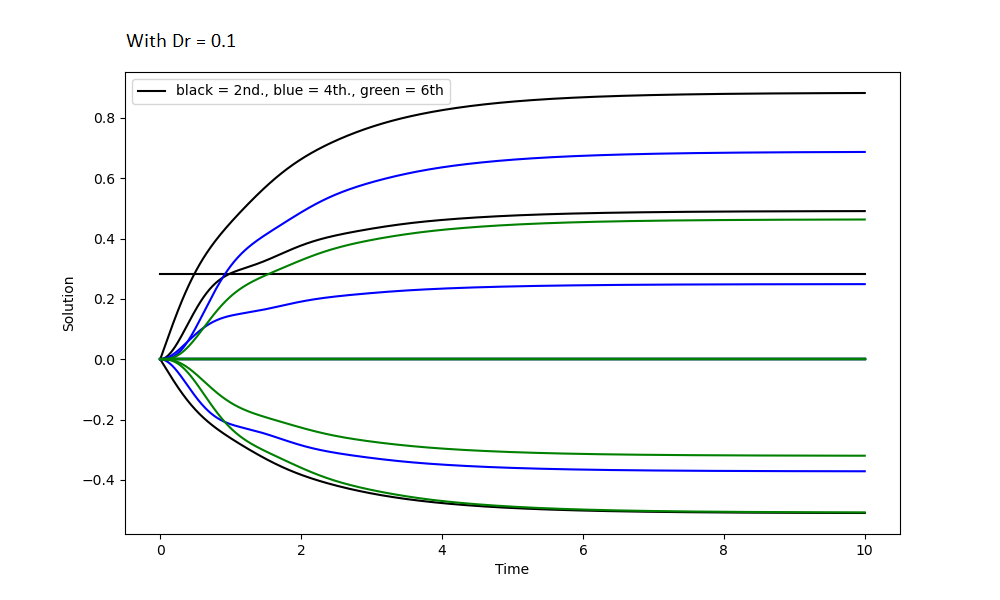
\includegraphics[width=\linewidth]{Bilder/elongational_l=1_lsg_ueber_Zeit_6th}
		\end{subfigure}
		\hfill
		\begin{subfigure}{0.48\textwidth}
			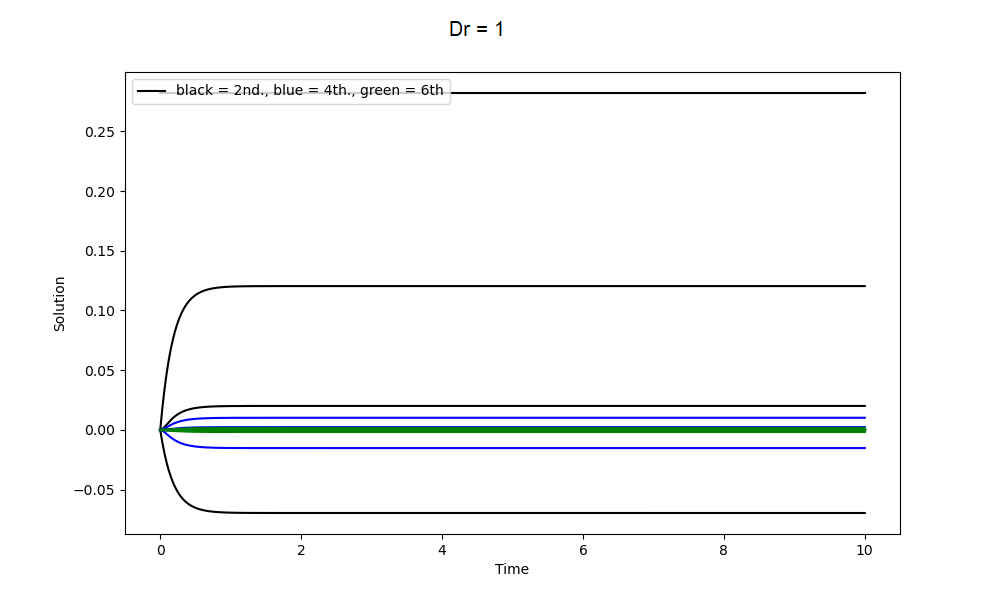
\includegraphics[width=\linewidth]{Bilder/elongational_l=1_lsg_ueber_Zeit_6th_dr=1}
		\end{subfigure}
		\caption{Coefficients as function of $6th$ order}
	\end{figure}
\end{frame}


\begin{frame}{Coefficients as function}
	\begin{figure}
		\begin{subfigure}{0.48\textwidth}
			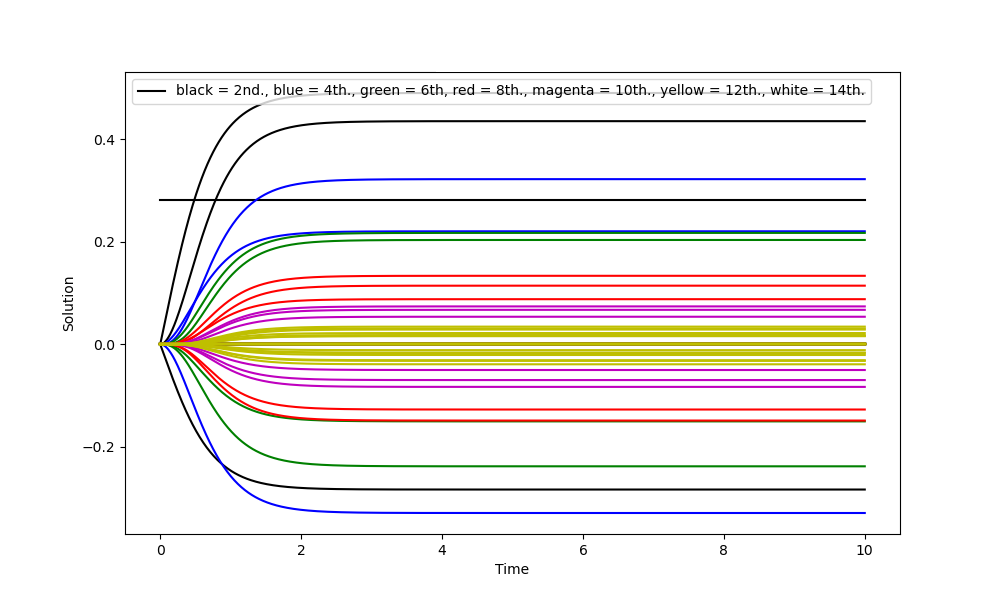
\includegraphics[width=\linewidth]{Bilder/elongational_l=1_lsg_ueber_Zeit_14th}
		\end{subfigure}
		\hfill
		\begin{subfigure}{0.48\textwidth}
			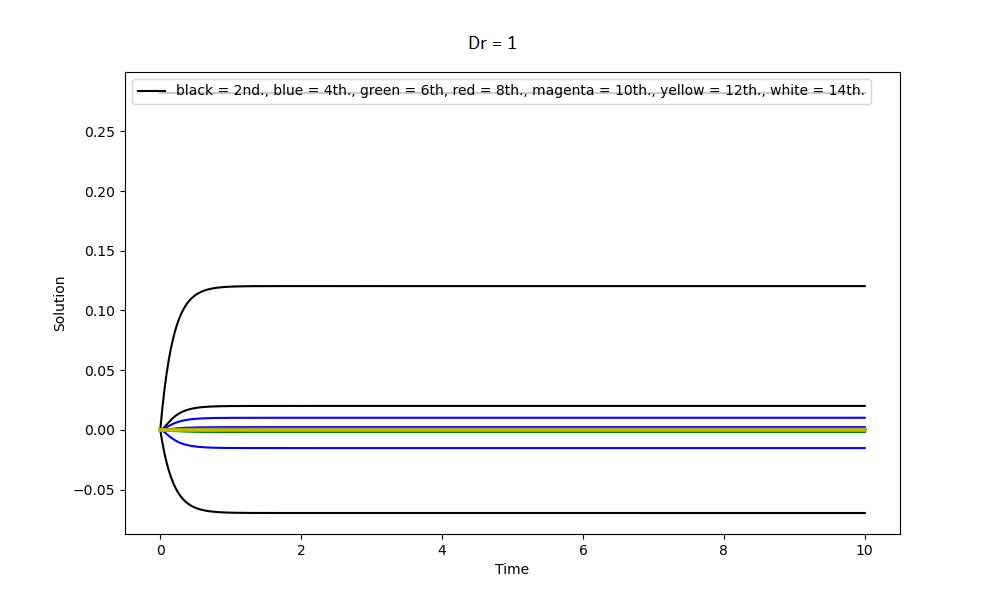
\includegraphics[width=\linewidth]{Bilder/elongational_l=1_lsg_ueber_Zeit_14th_dr=1}
		\end{subfigure}
		\caption{Coefficients as function of $14th$ order}
	\end{figure}
\end{frame}





%%%%%%%%%%%%%%%%%%%%%%%%%%%%%%%%%%%%%
%%%%%%%%%%%%%%%%%%%%%%%%%%%%%%%%%%%%%
% Shear flow on S^1
%%%%%%%%%%%%%%%%%%%%%%%%%%%%%%%%%%%%%
%%%%%%%%%%%%%%%%%%%%%%%%%%%%%%%%%%%%%

\begin{comment}
\subsection{Shear flow on $S^1$ and $S^2$}

\begin{frame}
	\centering
	Shear flow on $S^1$
\end{frame}

\begin{frame}{Shear flow on $S^1$}
	\scriptsize
	The externally imposed velocity gradient has the form
	\begin{figure}
	\centering
	\begin{equation}
	\nabla_{\mathbf{x}} \mathbf{u}=\begin{pmatrix}
		0 & 1 & 0 \\
		0 & 0 & 0 \\
		0 & 0 & 0
	\end{pmatrix}
	\end{equation}
	\end{figure}

TODO
\end{frame}

\subsubsection{Stability analysis}
\begin{frame}{Shear flow  on $S^1$: Stability analysis}
	\begin{figure}
		\centering
		\begin{minipage}{0.4\linewidth}
			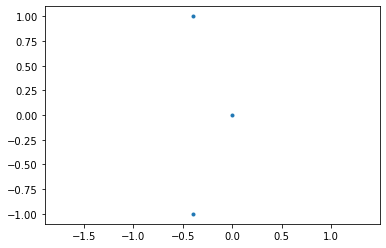
\includegraphics[scale=.42]{Bilder/Stability_analysis_shearflow_N=1_dr0.1}
		\end{minipage}
		\hspace{1cm}
		\begin{minipage}{0.4\linewidth}
			\centering
			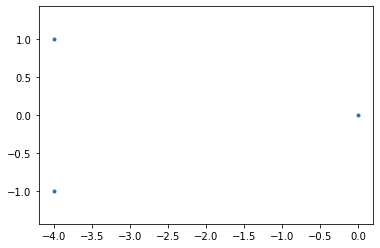
\includegraphics[scale=0.42]{Bilder/Stability_analysis_shearflow_N=1_dr1}
		\end{minipage}
		\caption{Eigenvalue of matrix $A$ with $N=1$}
	\end{figure}
	
	\begin{block}{Proposition 2}
		Sprectal method for $N=1$ is stable with for both small and large $D_r$.
	\end{block}
\end{frame}


\begin{frame}{Shear flow  on $S^1$: Stability analysis}
	\begin{figure}
		\centering
		\begin{minipage}{0.4\linewidth}
			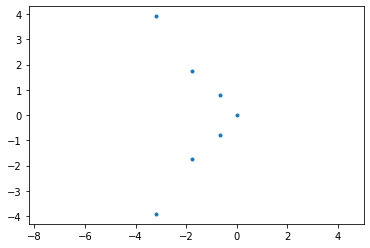
\includegraphics[scale=.42]{Bilder/Stability_analysis_shearflow_N=3_dr0.1}
		\end{minipage}
		\hspace{1cm}
		\begin{minipage}{0.4\linewidth}
			\centering
			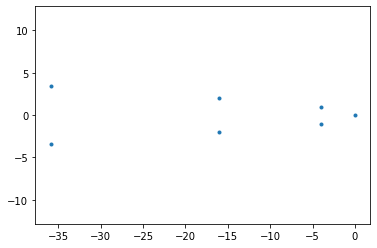
\includegraphics[scale=0.42]{Bilder/Stability_analysis_shearflow_N=3_dr1}
		\end{minipage}
		\caption{Eigenvalue of matrix $A$ $N=3$}
	\end{figure}
	
	\begin{block}{Proposition 3}
		Sprectal method for $N=3$ is stable with for both small and large $D_r$.
	\end{block}
\end{frame}
	Inhalt...
\end{comment}

%%%%%%%%%%%%%%%%%%%%%%%%%%%%%%%%%%%%%
%%%%%%%%%%%%%%%%%%%%%%%%%%%%%%%%%%%%%
% Shear flow on S^2 
%%%%%%%%%%%%%%%%%%%%%%%%%%%%%%%%%%%%%
%%%%%%%%%%%%%%%%%%%%%%%%%%%%%%%%%%%%%


\begin{frame}
	\centering
	Shear flow on $S^2$
\end{frame}

\begin{frame}{Shear flow on $S^2$}
	\scriptsize
	Consider the externally imposed shear flow 
	\begin{figure}
		\centering
		\begin{equation}
			\mathbf{u}=\begin{pmatrix}
				u(y) \\
				0 \\
				0
			\end{pmatrix}, \quad \nabla_{\mathbf{x}} \mathbf{u}=\begin{pmatrix}
				0 & 1 & 0 \\
				0 & 0 & 0 \\
				0 & 0 & 0
			\end{pmatrix}
		\end{equation}
	\end{figure}

\begin{figure}
	\small
	\begin{minipage}{0.43\textwidth}
		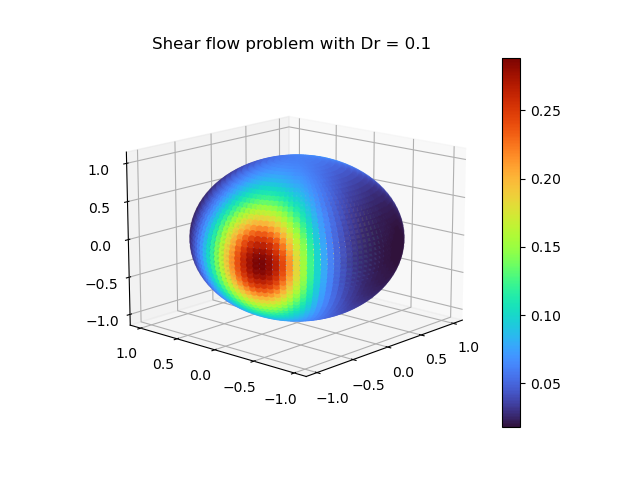
\includegraphics[scale=0.35]{Bilder/shearflow_12th_dr0.1}
	\end{minipage}
	\hfill 
	\begin{minipage}{0.43\textwidth}
		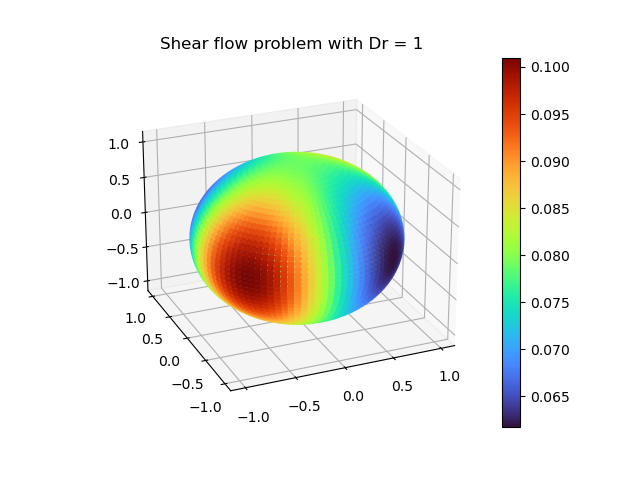
\includegraphics[scale=0.35]{Bilder/shearflow_12th_linspace(0,10,500)_dr=1}
	\end{minipage}
	\caption{Steady state solution of the Smoluchowski equation approximated at $T = 10$ using different values of $D_r$.}
\end{figure}
\end{frame}

\begin{frame}{Shear flow: Stability analysis}
	\begin{figure}
		\centering
		\begin{minipage}{0.4\linewidth}
			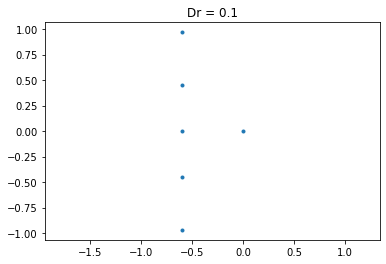
\includegraphics[scale=.42]{Bilder/Stability_analysis_shearflow_2nd_dr0.1}
		\end{minipage}
		\hspace{1cm}
		\begin{minipage}{0.4\linewidth}
			\centering
			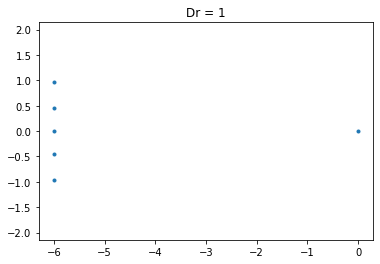
\includegraphics[scale=0.42]{Bilder/Stability_analysis_shearflow_2nd_dr1}
		\end{minipage}
		\caption{Eigenvalue of matrix $A$ with basis functions of $2nd$ order}
	\end{figure}
	
	\begin{block}{Finding}
		Sprectal method for $2nd$ order is stable with for both small and large $D_r$.
	\end{block}
\end{frame}

\begin{frame}{Shear flow: Stability analysis}
	\begin{figure}
		\centering
		\begin{minipage}{0.4\linewidth}
			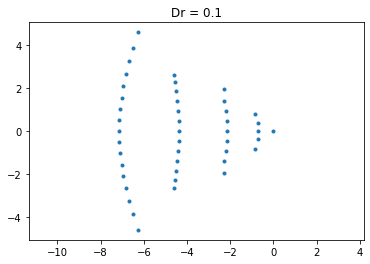
\includegraphics[scale=.42]{Bilder/Stability_analysis_shearflow_8th_dr0.1}
		\end{minipage}
		\hspace{1cm}
		\begin{minipage}{0.4\linewidth}
			\centering
			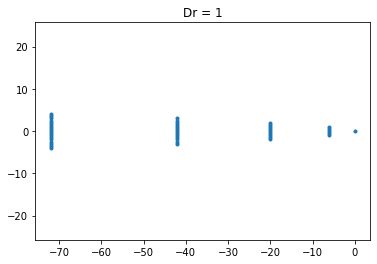
\includegraphics[scale=0.42]{Bilder/Stability_analysis_shearflow_8th_dr1}
		\end{minipage}
		\caption{Eigenvalue of matrix $A$ with basis functions of $8th$ order}
	\end{figure}
	
	\begin{block}{Proposition 2}
		Sprectal method for $8th$ order is stable with for both small and large $D_r$.
	\end{block}
\end{frame}



%%%%%%%%%%%%%%%%%%%%%%%%%%%%%%%%%%



\begin{comment}
\begin{frame}{Elongational flow: Stability analysis}
	\begin{columns}
		\begin{column}{0.5\textwidth}
			\begin{figure}
				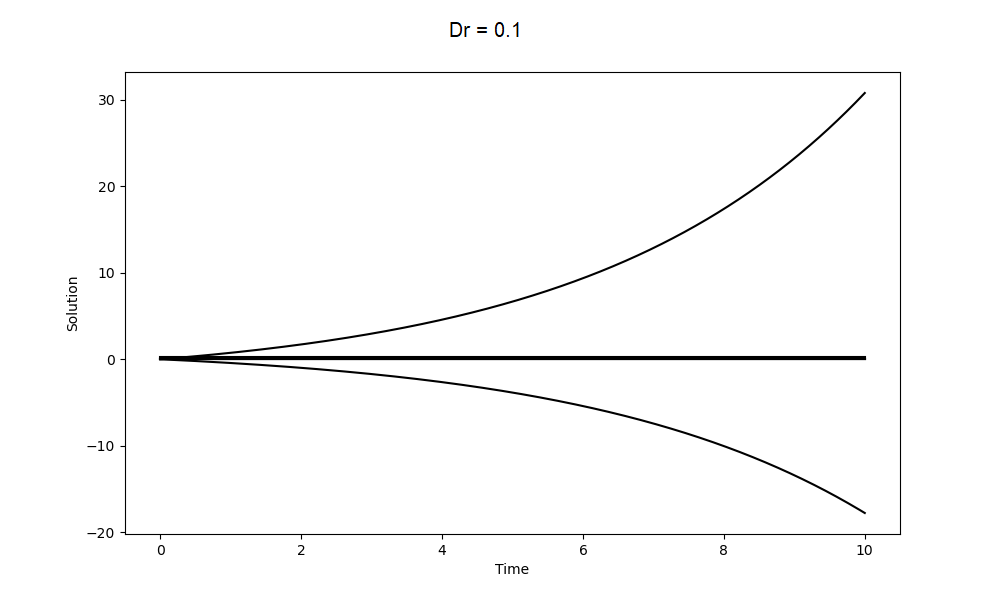
\includegraphics[width=0.97\linewidth]{Bilder/elongational_l=1_lsg_ueber_Zeit_2nd}
				\caption{Coefficients as function of time}
			\end{figure}
		\end{column}
		\begin{column}{0.5\textwidth}
			\begin{figure}
				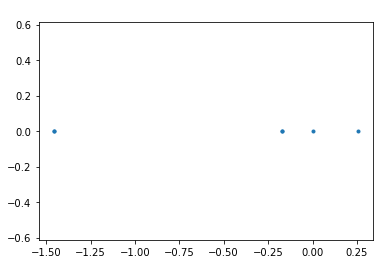
\includegraphics[width=0.8\linewidth]{Bilder/Stability_analysis_2nd_dr0.1}
				\caption{Eigenvalue of matrix $A$}
			\end{figure}
		\end{column}
	\end{columns}
	\centering
	With $2nd.$ order and $D_r = 0.1$.
\end{frame}

\begin{frame}{Elongational flow: Stability analysis}
	\begin{columns}
		\begin{column}{0.5\textwidth}
			\begin{figure}
				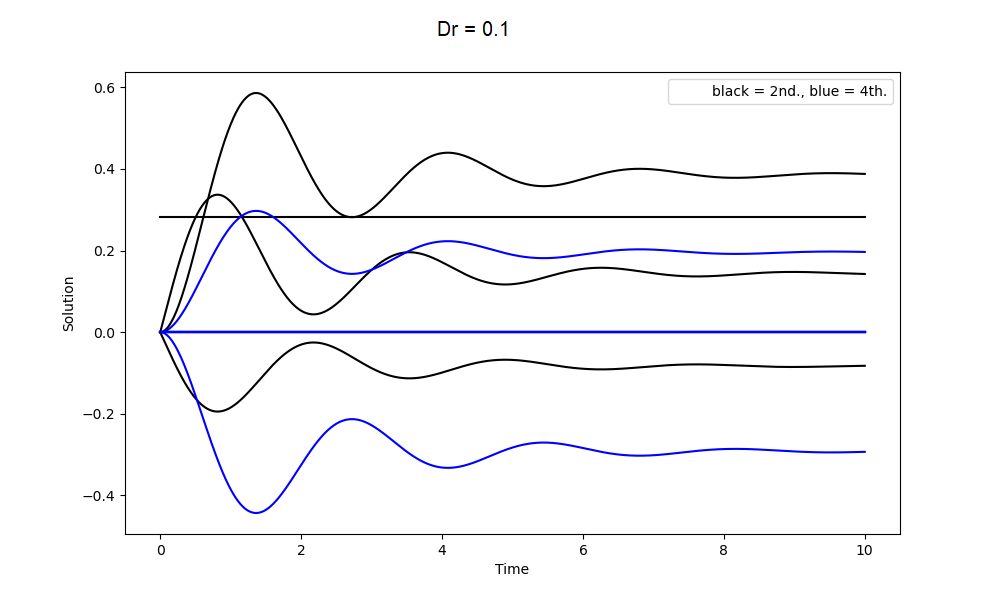
\includegraphics[width=0.97\linewidth]{Bilder/elongational_l=1_lsg_ueber_Zeit_4th}
				\caption{Coefficients as function of time}
			\end{figure}
		\end{column}
		\begin{column}{0.5\textwidth}
			\begin{figure}
				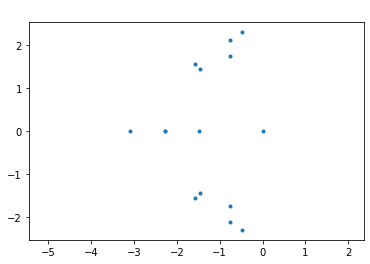
\includegraphics[width=0.8\linewidth]{Bilder/Stability_analysis_4th_dr0.1}
				\caption{Eigenvalue of matrix $A$}
			\end{figure}
		\end{column}
	\end{columns}
	\centering
	With $4th.$ order and $D_r = 0.1$.
\end{frame}


\begin{frame}{Elongational flow: Stability analysis}
	\begin{columns}
		\begin{column}{0.5\textwidth}
			\begin{figure}
				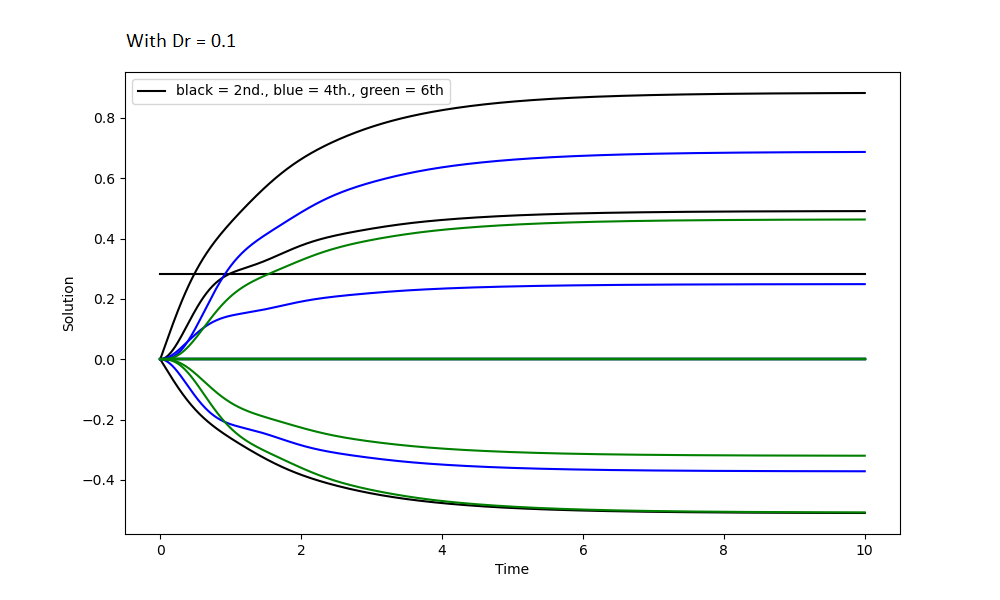
\includegraphics[width=0.97\linewidth]{Bilder/elongational_l=1_lsg_ueber_Zeit_6th}
				\caption{Coefficients as function of time}
			\end{figure}
		\end{column}
		\begin{column}{0.5\textwidth}
			\begin{figure}
				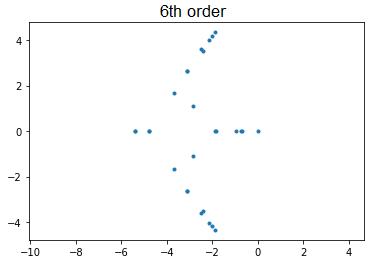
\includegraphics[width=0.82\linewidth]{Bilder/Stability_analysis_6th_dr0.1}
				\caption{Eigenvalue of matrix $A$}
			\end{figure}
		\end{column}
	\end{columns}
	\centering
	With $6th.$ order and $D_r = 0.1$.
\end{frame}

\begin{frame}{Elongational flow: Stability analysis}
	\begin{columns}
		\begin{column}{0.5\textwidth}
			\begin{figure}
				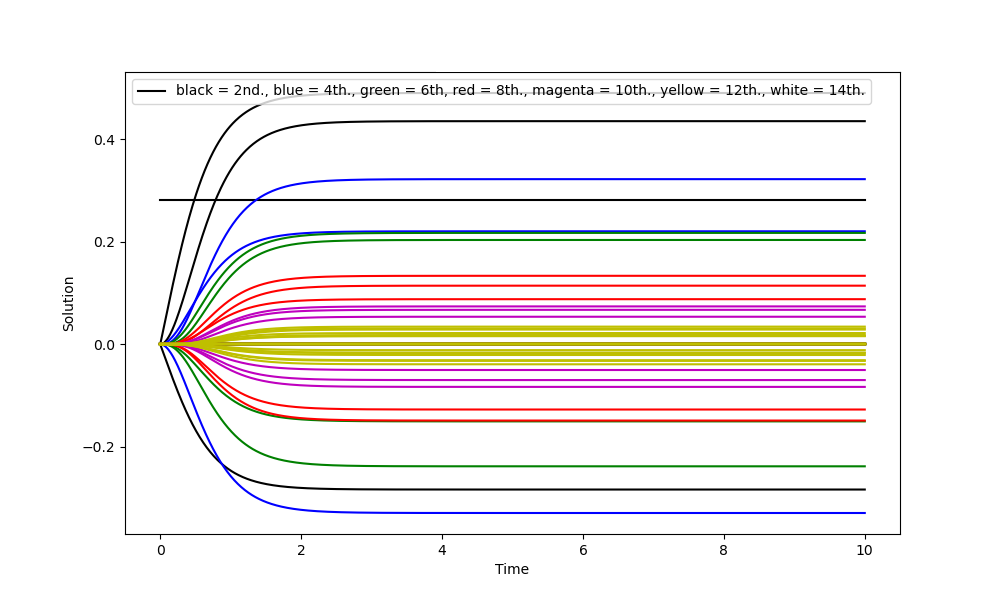
\includegraphics[width=0.97\linewidth]{Bilder/elongational_l=1_lsg_ueber_Zeit_14th}
				\caption{Coefficients as function of time}
			\end{figure}
		\end{column}
		\begin{column}{0.5\textwidth}
			\begin{figure}
				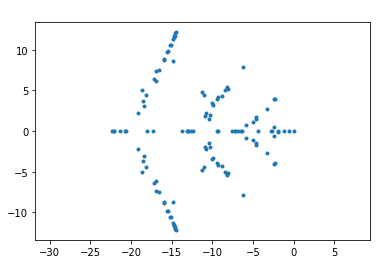
\includegraphics[width=0.83\linewidth]{Bilder/Stability_analysis_14th_dr0.1}
				\caption{Eigenvalue of matrix $A$}
			\end{figure}
		\end{column}
	\end{columns}
	\centering
	With $14th.$ order and $D_r = 0.1$.
\end{frame}
\end{comment}


\begin{comment}
\begin{frame}{Elongational flow: Stability analysis}
	\begin{figure}
		\centering
		\begin{minipage}{0.4\linewidth}
			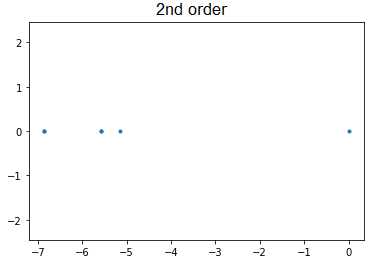
\includegraphics[scale=.42]{Bilder/Stability_analysis_2nd_dr1}
		\end{minipage}
		\hspace{1cm}
		\begin{minipage}{0.4\linewidth}
			\centering
			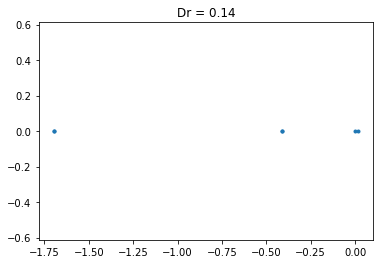
\includegraphics[scale=0.42]{Bilder/Stability_analysis_2nd_dr0.14}
		\end{minipage}
		\caption{Eigenvalue of matrix $A$ with basis functions of $2nd.$ order}
	\end{figure}
	
	\begin{block}{Finding 1}
		The maximum value of eigenvalue of matrix $A$ with basis functions of $2nd.$ order is $0.01714 > 0$. It follows:
		Sprectal method for $2nd.$ order is unstable with $D_r < 0.15$.
	\end{block}
\end{frame}
\end{comment}


\begin{frame}{Conclusion}
		\begin{itemize}
			\item Derivation of the sprectal method is the first step to derive the moment system
			\item In order for the method is stable,
				\begin{itemize}
					\item for small $D_r$ more approach functions 
					\item for large $D_r$ smaller time steps 
				\end{itemize} 
			is needed
		\end{itemize}
\end{frame}


%\begin{frame}
%	\begin{figure}[h]
%		\centering
%		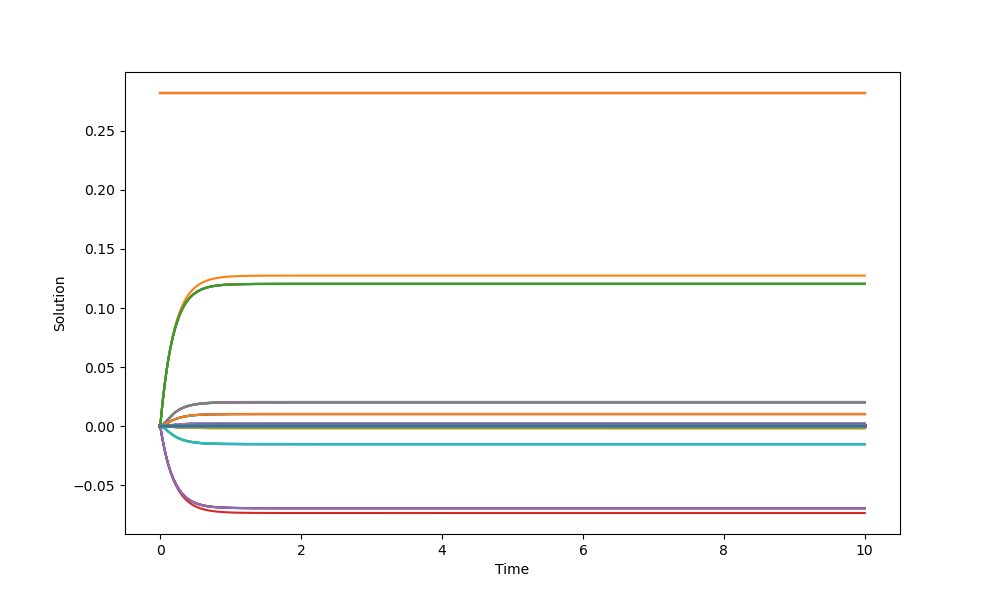
\includegraphics[scale=.35]{Bilder/Solution_over_time_14th}
%		\caption{Numerical solution of ODE systems over time with $D_r$ = 1}
%		\label{fig: Solution of ODE systems over time with $D_r$ = 1}
%	\end{figure}
%\end{frame}

